
%% bare_jrnl.tex
%% V1.4b
%% 2015/08/26
%% by Michael Shell
%% see http://www.michaelshell.org/
%% for current contact information.
%%
%% This is a skeleton file demonstrating the use of IEEEtran.cls
%% (requires IEEEtran.cls version 1.8b or later) with an IEEE
%% journal paper.
%%
%% Support sites:
%% http://www.michaelshell.org/tex/ieeetran/
%% http://www.ctan.org/pkg/ieeetran
%% and
%% http://www.ieee.org/

%%*************************************************************************
%% Legal Notice:
%% This code is offered as-is without any warranty either expressed or
%% implied; without even the implied warranty of MERCHANTABILITY or
%% FITNESS FOR A PARTICULAR PURPOSE! 
%% User assumes all risk.
%% In no event shall the IEEE or any contributor to this code be liable for
%% any damages or losses, including, but not limited to, incidental,
%% consequential, or any other damages, resulting from the use or misuse
%% of any information contained here.
%%
%% All comments are the opinions of their respective authors and are not
%% necessarily endorsed by the IEEE.
%%
%% This work is distributed under the LaTeX Project Public License (LPPL)
%% ( http://www.latex-project.org/ ) version 1.3, and may be freely used,
%% distributed and modified. A copy of the LPPL, version 1.3, is included
%% in the base LaTeX documentation of all distributions of LaTeX released
%% 2003/12/01 or later.
%% Retain all contribution notices and credits.
%% ** Modified files should be clearly indicated as such, including  **
%% ** renaming them and changing author support contact information. **
%%*************************************************************************


% *** Authors should verify (and, if needed, correct) their LaTeX system  ***
% *** with the testflow diagnostic prior to trusting their LaTeX platform ***
% *** with production work. The IEEE's font choices and paper sizes can   ***
% *** trigger bugs that do not appear when using other class files.       ***                          ***
% The testflow support page is at:
% http://www.michaelshell.org/tex/testflow/



\documentclass[journal]{IEEEtran}
%
% If IEEEtran.cls has not been installed into the LaTeX system files,
% manually specify the path to it like:
% \documentclass[journal]{../sty/IEEEtran}


\usepackage{cite}
\usepackage{amsmath,amssymb,amsfonts}
\usepackage{algorithmic}
\usepackage{graphicx}
\usepackage{textcomp}
\usepackage{xcolor}

\usepackage{pgfplots} % per a graficar amb LaTeX
\pgfplotsset{samples=2000} % número màxim de punts d'una corba que genera ell, canviar
\pgfplotsset{compat=1.16} % perquè si no el pgfplot dóna error
\usepackage{import} % per a les imatges d'Inkscape
\usepackage{xifthen} % per a les imatges d'Inkscape
\usepackage{pdfpages} % per a les imatges d'Inkscape
\usepackage{transparent} % per a les imatges d'Inkscape
\usepackage[RPvoltages]{circuitikz} % per tal que no salti warning
\usetikzlibrary{arrows, decorations.markings, arrows.meta} % per a dibuixar fletxes d'intensitat
\usepackage{balance}
%\usepackage{flushend}
\usepackage{lettrine}


% Some very useful LaTeX packages include:
% (uncomment the ones you want to load)


% *** MISC UTILITY PACKAGES ***
%
%\usepackage{ifpdf}
% Heiko Oberdiek's ifpdf.sty is very useful if you need conditional
% compilation based on whether the output is pdf or dvi.
% usage:
% \ifpdf
%   % pdf code
% \else
%   % dvi code
% \fi
% The latest version of ifpdf.sty can be obtained from:
% http://www.ctan.org/pkg/ifpdf
% Also, note that IEEEtran.cls V1.7 and later provides a builtin
% \ifCLASSINFOpdf conditional that works the same way.
% When switching from latex to pdflatex and vice-versa, the compiler may
% have to be run twice to clear warning/error messages.






% *** CITATION PACKAGES ***
%
%\usepackage{cite}
% cite.sty was written by Donald Arseneau
% V1.6 and later of IEEEtran pre-defines the format of the cite.sty package
% \cite{} output to follow that of the IEEE. Loading the cite package will
% result in citation numbers being automatically sorted and properly
% "compressed/ranged". e.g., [1], [9], [2], [7], [5], [6] without using
% cite.sty will become [1], [2], [5]--[7], [9] using cite.sty. cite.sty's
% \cite will automatically add leading space, if needed. Use cite.sty's
% noadjust option (cite.sty V3.8 and later) if you want to turn this off
% such as if a citation ever needs to be enclosed in parenthesis.
% cite.sty is already installed on most LaTeX systems. Be sure and use
% version 5.0 (2009-03-20) and later if using hyperref.sty.
% The latest version can be obtained at:
% http://www.ctan.org/pkg/cite
% The documentation is contained in the cite.sty file itself.






% *** GRAPHICS RELATED PACKAGES ***
%
\ifCLASSINFOpdf
  % \usepackage[pdftex]{graphicx}
  % declare the path(s) where your graphic files are
  % \graphicspath{{../pdf/}{../jpeg/}}
  % and their extensions so you won't have to specify these with
  % every instance of \includegraphics
  % \DeclareGraphicsExtensions{.pdf,.jpeg,.png}
\else
  % or other class option (dvipsone, dvipdf, if not using dvips). graphicx
  % will default to the driver specified in the system graphics.cfg if no
  % driver is specified.
  % \usepackage[dvips]{graphicx}
  % declare the path(s) where your graphic files are
  % \graphicspath{{../eps/}}
  % and their extensions so you won't have to specify these with
  % every instance of \includegraphics
  % \DeclareGraphicsExtensions{.eps}
\fi
% graphicx was written by David Carlisle and Sebastian Rahtz. It is
% required if you want graphics, photos, etc. graphicx.sty is already
% installed on most LaTeX systems. The latest version and documentation
% can be obtained at: 
% http://www.ctan.org/pkg/graphicx
% Another good source of documentation is "Using Imported Graphics in
% LaTeX2e" by Keith Reckdahl which can be found at:
% http://www.ctan.org/pkg/epslatex
%
% latex, and pdflatex in dvi mode, support graphics in encapsulated
% postscript (.eps) format. pdflatex in pdf mode supports graphics
% in .pdf, .jpeg, .png and .mps (metapost) formats. Users should ensure
% that all non-photo figures use a vector format (.eps, .pdf, .mps) and
% not a bitmapped formats (.jpeg, .png). The IEEE frowns on bitmapped formats
% which can result in "jaggedy"/blurry rendering of lines and letters as
% well as large increases in file sizes.
%
% You can find documentation about the pdfTeX application at:
% http://www.tug.org/applications/pdftex





% *** MATH PACKAGES ***
%
%\usepackage{amsmath}
% A popular package from the American Mathematical Society that provides
% many useful and powerful commands for dealing with mathematics.
%
% Note that the amsmath package sets \interdisplaylinepenalty to 10000
% thus preventing page breaks from occurring within multiline equations. Use:
%\interdisplaylinepenalty=2500
% after loading amsmath to restore such page breaks as IEEEtran.cls normally
% does. amsmath.sty is already installed on most LaTeX systems. The latest
% version and documentation can be obtained at:
% http://www.ctan.org/pkg/amsmath





% *** SPECIALIZED LIST PACKAGES ***
%
%\usepackage{algorithmic}
% algorithmic.sty was written by Peter Williams and Rogerio Brito.
% This package provides an algorithmic environment fo describing algorithms.
% You can use the algorithmic environment in-text or within a figure
% environment to provide for a floating algorithm. Do NOT use the algorithm
% floating environment provided by algorithm.sty (by the same authors) or
% algorithm2e.sty (by Christophe Fiorio) as the IEEE does not use dedicated
% algorithm float types and packages that provide these will not provide
% correct IEEE style captions. The latest version and documentation of
% algorithmic.sty can be obtained at:
% http://www.ctan.org/pkg/algorithms
% Also of interest may be the (relatively newer and more customizable)
% algorithmicx.sty package by Szasz Janos:
% http://www.ctan.org/pkg/algorithmicx




% *** ALIGNMENT PACKAGES ***
%
%\usepackage{array}
% Frank Mittelbach's and David Carlisle's array.sty patches and improves
% the standard LaTeX2e array and tabular environments to provide better
% appearance and additional user controls. As the default LaTeX2e table
% generation code is lacking to the point of almost being broken with
% respect to the quality of the end results, all users are strongly
% advised to use an enhanced (at the very least that provided by array.sty)
% set of table tools. array.sty is already installed on most systems. The
% latest version and documentation can be obtained at:
% http://www.ctan.org/pkg/array


% IEEEtran contains the IEEEeqnarray family of commands that can be used to
% generate multiline equations as well as matrices, tables, etc., of high
% quality.




% *** SUBFIGURE PACKAGES ***
%\ifCLASSOPTIONcompsoc
%  \usepackage[caption=false,font=normalsize,labelfont=sf,textfont=sf]{subfig}
%\else
%  \usepackage[caption=false,font=footnotesize]{subfig}
%\fi
% subfig.sty, written by Steven Douglas Cochran, is the modern replacement
% for subfigure.sty, the latter of which is no longer maintained and is
% incompatible with some LaTeX packages including fixltx2e. However,
% subfig.sty requires and automatically loads Axel Sommerfeldt's caption.sty
% which will override IEEEtran.cls' handling of captions and this will result
% in non-IEEE style figure/table captions. To prevent this problem, be sure
% and invoke subfig.sty's "caption=false" package option (available since
% subfig.sty version 1.3, 2005/06/28) as this is will preserve IEEEtran.cls
% handling of captions.
% Note that the Computer Society format requires a larger sans serif font
% than the serif footnote size font used in traditional IEEE formatting
% and thus the need to invoke different subfig.sty package options depending
% on whether compsoc mode has been enabled.
%
% The latest version and documentation of subfig.sty can be obtained at:
% http://www.ctan.org/pkg/subfig




% *** FLOAT PACKAGES ***
%
%\usepackage{fixltx2e}
% fixltx2e, the successor to the earlier fix2col.sty, was written by
% Frank Mittelbach and David Carlisle. This package corrects a few problems
% in the LaTeX2e kernel, the most notable of which is that in current
% LaTeX2e releases, the ordering of single and double column floats is not
% guaranteed to be preserved. Thus, an unpatched LaTeX2e can allow a
% single column figure to be placed prior to an earlier double column
% figure.
% Be aware that LaTeX2e kernels dated 2015 and later have fixltx2e.sty's
% corrections already built into the system in which case a warning will
% be issued if an attempt is made to load fixltx2e.sty as it is no longer
% needed.
% The latest version and documentation can be found at:
% http://www.ctan.org/pkg/fixltx2e


%\usepackage{stfloats}
% stfloats.sty was written by Sigitas Tolusis. This package gives LaTeX2e
% the ability to do double column floats at the bottom of the page as well
% as the top. (e.g., "\begin{figure*}[!b]" is not normally possible in
% LaTeX2e). It also provides a command:
%\fnbelowfloat
% to enable the placement of footnotes below bottom floats (the standard
% LaTeX2e kernel puts them above bottom floats). This is an invasive package
% which rewrites many portions of the LaTeX2e float routines. It may not work
% with other packages that modify the LaTeX2e float routines. The latest
% version and documentation can be obtained at:
% http://www.ctan.org/pkg/stfloats
% Do not use the stfloats baselinefloat ability as the IEEE does not allow
% \baselineskip to stretch. Authors submitting work to the IEEE should note
% that the IEEE rarely uses double column equations and that authors should try
% to avoid such use. Do not be tempted to use the cuted.sty or midfloat.sty
% packages (also by Sigitas Tolusis) as the IEEE does not format its papers in
% such ways.
% Do not attempt to use stfloats with fixltx2e as they are incompatible.
% Instead, use Morten Hogholm'a dblfloatfix which combines the features
% of both fixltx2e and stfloats:
%
% \usepackage{dblfloatfix}
% The latest version can be found at:
% http://www.ctan.org/pkg/dblfloatfix




%\ifCLASSOPTIONcaptionsoff
%  \usepackage[nomarkers]{endfloat}
% \let\MYoriglatexcaption\caption
% \renewcommand{\caption}[2][\relax]{\MYoriglatexcaption[#2]{#2}}
%\fi
% endfloat.sty was written by James Darrell McCauley, Jeff Goldberg and 
% Axel Sommerfeldt. This package may be useful when used in conjunction with 
% IEEEtran.cls'  captionsoff option. Some IEEE journals/societies require that
% submissions have lists of figures/tables at the end of the paper and that
% figures/tables without any captions are placed on a page by themselves at
% the end of the document. If needed, the draftcls IEEEtran class option or
% \CLASSINPUTbaselinestretch interface can be used to increase the line
% spacing as well. Be sure and use the nomarkers option of endfloat to
% prevent endfloat from "marking" where the figures would have been placed
% in the text. The two hack lines of code above are a slight modification of
% that suggested by in the endfloat docs (section 8.4.1) to ensure that
% the full captions always appear in the list of figures/tables - even if
% the user used the short optional argument of \caption[]{}.
% IEEE papers do not typically make use of \caption[]'s optional argument,
% so this should not be an issue. A similar trick can be used to disable
% captions of packages such as subfig.sty that lack options to turn off
% the subcaptions:
% For subfig.sty:
% \let\MYorigsubfloat\subfloat
% \renewcommand{\subfloat}[2][\relax]{\MYorigsubfloat[]{#2}}
% However, the above trick will not work if both optional arguments of
% the \subfloat command are used. Furthermore, there needs to be a
% description of each subfigure *somewhere* and endfloat does not add
% subfigure captions to its list of figures. Thus, the best approach is to
% avoid the use of subfigure captions (many IEEE journals avoid them anyway)
% and instead reference/explain all the subfigures within the main caption.
% The latest version of endfloat.sty and its documentation can obtained at:
% http://www.ctan.org/pkg/endfloat
%
% The IEEEtran \ifCLASSOPTIONcaptionsoff conditional can also be used
% later in the document, say, to conditionally put the References on a 
% page by themselves.




% *** PDF, URL AND HYPERLINK PACKAGES ***
%
%\usepackage{url}
% url.sty was written by Donald Arseneau. It provides better support for
% handling and breaking URLs. url.sty is already installed on most LaTeX
% systems. The latest version and documentation can be obtained at:
% http://www.ctan.org/pkg/url
% Basically, \url{my_url_here}.




% *** Do not adjust lengths that control margins, column widths, etc. ***
% *** Do not use packages that alter fonts (such as pslatex).         ***
% There should be no need to do such things with IEEEtran.cls V1.6 and later.
% (Unless specifically asked to do so by the journal or conference you plan
% to submit to, of course. )


% correct bad hyphenation here
\hyphenation{op-tical net-works semi-conduc-tor}


\begin{document}
%
% paper title
% Titles are generally capitalized except for words such as a, an, and, as,
% at, but, by, for, in, nor, of, on, or, the, to and up, which are usually
% not capitalized unless they are the first or last word of the title.
% Linebreaks \\ can be used within to get better formatting as desired.
% Do not put math or special symbols in the title.
\title{Alternative Approach to the Holomorphic Embedding Load-Flow Method}
%
%
% author names and IEEE memberships
% note positions of commas and nonbreaking spaces ( ~ ) LaTeX will not break
% a structure at a ~ so this keeps an author's name from being broken across
% two lines.
% use \thanks{} to gain access to the first footnote area
% a separate \thanks must be used for each paragraph as LaTeX2e's \thanks
% was not built to handle multiple paragraphs
%

\author{Josep Fanals i Batllori,~\IEEEmembership{Student Member,~IEEE,}
       and Sergio Herraiz Jaramillo%
% \thanks{M. Shell was with the Department
% of Electrical and Computer Engineering, Georgia Institute of Technology, Atlanta,
% GA, 30332 USA e-mail: (see http://www.michaelshell.org/contact.html).}% <-this % stops a space
\thanks{J. Fanals i Batllori is with Universitat de Girona, 17003 Girona, Spain, (e-mail: jfanals13@gmail.com)}% <-this % stops a space
\thanks{S. Herraiz Jaramillo is with the Department of Electrical, Electronical and Automatic Engineering, Universitat de Girona, 17003 Girona, Spain (e-mail: sergio.herraiz@udg.edu)}}

% note the % following the last \IEEEmembership and also \thanks - 
% these prevent an unwanted space from occurring between the last author name
% and the end of the author line. i.e., if you had this:
% 
% \author{....lastname \thanks{...} \thanks{...} }
%                     ^------------^------------^----Do not want these spaces!
%
% a space would be appended to the last name and could cause every name on that
% line to be shifted left slightly. This is one of those "LaTeX things". For
% instance, "\textbf{A} \textbf{B}" will typeset as "A B" not "AB". To get
% "AB" then you have to do: "\textbf{A}\textbf{B}"
% \thanks is no different in this regard, so shield the last } of each \thanks
% that ends a line with a % and do not let a space in before the next \thanks.
% Spaces after \IEEEmembership other than the last one are OK (and needed) as
% you are supposed to have spaces between the names. For what it is worth,
% this is a minor point as most people would not even notice if the said evil
% space somehow managed to creep in.



% The paper headers
\markboth{IEEE Transactions on Power Systems, Vol. XX, No. XX, XX 2020}{}%
% {Shell \MakeLowercase{\textit{et al.}}: Bare Demo of IEEEtran.cls for IEEE Journals}
% The only time the second header will appear is for the odd numbered pages
% after the title page when using the twoside option.
% 
% *** Note that you probably will NOT want to include the author's ***
% *** name in the headers of peer review papers.                   ***
% You can use \ifCLASSOPTIONpeerreview for conditional compilation here if
% you desire.




% If you want to put a publisher's ID mark on the page you can do it like
% this:
%\IEEEpubid{0000--0000/00\$00.00~\copyright~2015 IEEE}
% Remember, if you use this you must call \IEEEpubidadjcol in the second
% column for its text to clear the IEEEpubid mark.



% use for special paper notices
%\IEEEspecialpapernotice{(Invited Paper)}




% make the title area
\maketitle

% As a general rule, do not put math, special symbols or citations
% in the abstract or keywords.
\begin{abstract}
The Holomorphic Embedding Load-Flow Method is a novel recursive technique for solving the power flow of an electrical power system. Contrary to the traditional iterative schemes, it embeds the equations in a bigger problem from where the solution is then built. 
There is a wide range of possibilities to adapt the equations to the holomorphic embedding method. Although the so-called canonical embedding prevails as the most popular one, achieving the desired reference state may result in overcomplicating the algorithm.
This paper covers a simple alternative embedding, capable of offering adequate convergence properties, sometimes even faster than the canonical embedding. An 11-bus ill-conditioned system is studied in order to show that improvement. Furthermore, despite the fact that unique tools such as Sigma and Thévenin approximants were constructed with the canonical embedding in mind, they become fully compatible with the alternative embedding thanks to minor modifications. They are applied to the IEEE 30-bus system to display its functionality.
\end{abstract}

% Note that keywords are not normally used for peerreview papers.
\begin{IEEEkeywords}
holomorphic embedding method, load flow, power system analysis computing, power system simulation, Sigma approximants, Thévenin approximants.
\end{IEEEkeywords}






% For peer review papers, you can put extra information on the cover
% page as needed:
% \ifCLASSOPTIONpeerreview
% \begin{center} \bfseries EDICS Category: 3-BBND \end{center}
% \fi
%
% For peerreview papers, this IEEEtran command inserts a page break and
% creates the second title. It will be ignored for other modes.
\IEEEpeerreviewmaketitle



\section{Introduction}
% The very first letter is a 2 line initial drop letter followed
% by the rest of the first word in caps.
% 
% form to use if the first word consists of a single letter:
% \IEEEPARstart{A}{demo} file is ....
% 
% form to use if you need the single drop letter followed by
% normal text (unknown if ever used by the IEEE):
% \IEEEPARstart{A}{}demo file is ....
% 
% Some journals put the first two words in caps:
% \IEEEPARstart{T}{his demo} file is ....
% 
% Here we have the typical use of a "T" for an initial drop letter
% and "HIS" in caps to complete the first word.
\IEEEPARstart{P}{ower} flow or load flow is likely the most relevant problem concerning power systems. It describes the steady-state operation of the grid, which means that voltages, currents and powers are completely known. Unfortunately, it is a well-known fact that the equations involved are nonlinear.
% You must have at least 2 lines in the paragraph with the drop letter
% (should never be an issue)
Because of that, power flow calculations have been usually performed by iterative methods, such as the Gauss-Seidel and mostly the Newton-Raphson and its variations \cite{Novel},\cite{gomez}, with the fast decoupled load flow being one of them \cite{Stott}. The Newton-Raphson method converges quadratically. That causes it to converge to an acceptable solution with few iterations.

However, iterative methods are not guaranteed to always obtain the right solution. There are two main problems that the Newton-Raphson method and similar approaches have to face: one being the divergence of the solution, and the other, the convergence to an infeasible operating point \cite{Novel}. 

That is where the holomorphic embedding method comes into play. When the power flow is solvable, the method reaches the correct solution, whereas when the power flow is impossible to solve, the method signals it \cite{Trias2012},\cite{Trias2018},\cite{Trias_sigma}. The holomorphic embedding is based on, as the name suggests, submerging the original problem in a larger problem. When some reference conditions are provided, it is then able to compute the solution \cite{Trias2018}.

The choice of embedding is not unique \cite{Novel},\cite{Trias2018},\cite{TriasMarin},\cite{Schmidt}. The most notorious one looks for a reference state where the first coefficients of the unknowns are always the same, independent of the system \cite{Trias2018},\cite{Rao},\cite{Tylavsky3}. It will be referred to as the canonical embedding. Despite its relative complexity, not only it works properly, but it is also compatible with the totality of tools that the holomorphic embedding method has to offer. Probably the most prominent tools are Sigma and Thévenin approximants, detailed in \cite{Trias2018}. 

Some authors have opted for an approach slightly less complex \cite{Novel},\cite{Schmidt},\cite{subramanianPV}. The main trouble has to do with PV buses, where the injected reactive power is unknown. References \cite{Schmidt},\cite{Subramanian} worked with an implementation that manages to only consider the voltages as unknowns. Nonetheless, that embedding lacks robustness, as it presents convergence problems. That has been affirmed in \cite{Novel}, where the initialization is carried out with iterative methods, but in essence the procedure stays the same. 

To solve that, several embeddings are developed in \cite{wallace}. They successfully achieve smaller errors than \cite{subramanianPV},\cite{Subramanian}. Despite that, it can be argued that the embedding is somewhat complex, or at least, way different from the canonical embedding. The effects of tap changers are not mentioned and neither unique tools of the holomorphic embedding method like Sigma and Thévenin approximants are covered. 

This paper details an approach similar to the canonical embedding which turns out to be slightly simpler. Contrary to \cite{Novel},\cite{Schmidt},\cite{subramanianPV} its convergence properties are satisfactory, and in certain situations even better than the canonical embedding. Another advantage is its compatibility with Sigma and Thévenin approximants. 

The outline of this work is as follows: Section \ref{sec1} introduces the canonical embedding; Section \ref{sec2} presents the alternative embedding and details the algorithm that has to be employed; Section \ref{sec3} reviews the concept and the importance of Sigma approximants, describes the modification needed in order to make it compatible with the alternative embedding and then, compares it with the results obtained with the canonical embedding; Section \ref{sec4} depicts the formulation of Thévenin approximants, covers the changes and the steps that need to be taken as well as showing its usage and how well they match the values resulting from the canonical embedding; finally, Section \ref{sec5} concludes the paper.

% \subsection{Subsection Heading Here}
% Subsection text here.

% needed in second column of first page if using \IEEEpubid
%\IEEEpubidadjcol

% \subsubsection{Subsubsection Heading Here}
% Subsubsection text here.


% An example of a floating figure using the graphicx package.
% Note that \label must occur AFTER (or within) \caption.
% For figures, \caption should occur after the \includegraphics.
% Note that IEEEtran v1.7 and later has special internal code that
% is designed to preserve the operation of \label within \caption
% even when the captionsoff option is in effect. However, because
% of issues like this, it may be the safest practice to put all your
% \label just after \caption rather than within \caption{}.
%
% Reminder: the "draftcls" or "draftclsnofoot", not "draft", class
% option should be used if it is desired that the figures are to be
% displayed while in draft mode.
%
%\begin{figure}[!t]
%\centering
%\includegraphics[width=2.5in]{myfigure}
% where an .eps filename suffix will be assumed under latex, 
% and a .pdf suffix will be assumed for pdflatex; or what has been declared
% via \DeclareGraphicsExtensions.
%\caption{Simulation results for the network.}
%\label{fig_sim}
%\end{figure}

% Note that the IEEE typically puts floats only at the top, even when this
% results in a large percentage of a column being occupied by floats.


% An example of a double column floating figure using two subfigures.
% (The subfig.sty package must be loaded for this to work.)
% The subfigure \label commands are set within each subfloat command,
% and the \label for the overall figure must come after \caption.
% \hfil is used as a separator to get equal spacing.
% Watch out that the combined width of all the subfigures on a 
% line do not exceed the text width or a line break will occur.
%
%\begin{figure*}[!t]
%\centering
%\subfloat[Case I]{\includegraphics[width=2.5in]{box}%
%\label{fig_first_case}}
%\hfil
%\subfloat[Case II]{\includegraphics[width=2.5in]{box}%
%\label{fig_second_case}}
%\caption{Simulation results for the network.}
%\label{fig_sim}
%\end{figure*}
%
% Note that often IEEE papers with subfigures do not employ subfigure
% captions (using the optional argument to \subfloat[]), but instead will
% reference/describe all of them (a), (b), etc., within the main caption.
% Be aware that for subfig.sty to generate the (a), (b), etc., subfigure
% labels, the optional argument to \subfloat must be present. If a
% subcaption is not desired, just leave its contents blank,
% e.g., \subfloat[].


% An example of a floating table. Note that, for IEEE style tables, the
% \caption command should come BEFORE the table and, given that table
% captions serve much like titles, are usually capitalized except for words
% such as a, an, and, as, at, but, by, for, in, nor, of, on, or, the, to
% and up, which are usually not capitalized unless they are the first or
% last word of the caption. Table text will default to \footnotesize as
% the IEEE normally uses this smaller font for tables.
% The \label must come after \caption as always.
%
%\begin{table}[!t]
%% increase table row spacing, adjust to taste
%\renewcommand{\arraystretch}{1.3}
% if using array.sty, it might be a good idea to tweak the value of
% \extrarowheight as needed to properly center the text within the cells
%\caption{An Example of a Table}
%\label{table_example}
%\centering
%% Some packages, such as MDW tools, offer better commands for making tables
%% than the plain LaTeX2e tabular which is used here.
%\begin{tabular}{|c||c|}
%\hline
%One & Two\\
%\hline
%Three & Four\\
%\hline
%\end{tabular}
%\end{table}


% Note that the IEEE does not put floats in the very first column
% - or typically anywhere on the first page for that matter. Also,
% in-text middle ("here") positioning is typically not used, but it
% is allowed and encouraged for Computer Society conferences (but
% not Computer Society journals). Most IEEE journals/conferences use
% top floats exclusively. 
% Note that, LaTeX2e, unlike IEEE journals/conferences, places
% footnotes above bottom floats. This can be corrected via the
% \fnbelowfloat command of the stfloats package.



\section{Canonical embedding} \label{sec1}
The Holomorphic Embedding Load-Flow Method takes an initial equation of the form
\begin{equation}
  \sum_{j} Y_{ij}V_j + Y_i^{sh}V_i=\frac{S^*_i}{V^*_i},\label{eq:1}
\end{equation}
where $Y_{ij}$ is the $i,j$ element of the series admittances bus matrix, $V$ stands for voltage, $Y^{sh}_i$ represents the object that collects all shunt admittances and $S_i$ is the power injected at bus $i$. Current injections could also be considered, although they have been ignored with the idea to keep the algorithm simple.  

The idea behind the embedding is based on integrating the power flow problem into a much larger problem. Under these circumstances, the construction of the solution initiates from a well-defined reference state, from which one is then able to extend the solutions \cite{Trias2018}. The traditional embedding transforms \eqref{eq:1} into
\begin{equation}
   \sum_{j} Y_{ij}V_j(s) + sY_i^{sh}V_i(s)=s\frac{S^*_i}{V^*_i(s^*)},\label{eq:2}
\end{equation}
where $s$ is the complex variable and $V_i(s)$ is in essence a series that obeys the generic form
\begin{equation}
  C(s)=C[0]+sC[1]+s^2C[2]+...+C[n]=\sum_{k=0}^{n}s^kC[k],\label{eq:10}
\end{equation}
where $n$ represents an arbitrary depth, usually between 20 and 40. One has to calculate all terms step by step. Not only voltages, but also each and every unknown variable follows the structure of \eqref{eq:10}. The holomorphic embedding starts from a reference state, where $s=0$, and then, it looks for the final solution at $s=1$. 

While it is true that the embedding can be chosen freely, it has to validate the Cauchy-Riemann conditions. Due to that specific reason, the last term of \eqref{eq:2} is embedded as $V^*_i(s^*)$ and not as $V^*_i(s)$. Both the canonical and the alternative embedding described in this paper adhere to that.  

At this point not only PQ buses should be considered. In addition to them, power systems contain PV buses, where reactive power is treated as an unknown. The original embedded equations follow
\begin{equation}
   \sum_{j} Y_{ij}V_j(s) + sY_i^{sh}V_i(s)=\frac{sP_i-jQ_i(s)}{V^*_i(s^*)},\label{eq:3}
\end{equation}
where $P_i$ is the given active power and $Q_i(s)$ becomes the series with the reactive power coefficients. It has to be noted that the term $Q_i(s)$ does not multiply by $s$. That is critical because the initial solution (the one corresponding to the reference state) should emerge from a linear system of equations. 

The way to deviate from the mentioned inconvenience consists in establishing beforehand
\begin{equation}
  \begin{cases}
  V_i[0]=1 & i\in \text{PQ, PV, slack},\\
  Q_i[0]=0 & i\in \text{PV},
  \end{cases}
  \label{eq:4}
\end{equation}
where PQ, PV and slack are the sets containing their respective type of bus.

With the aim of forcing the initialization of $V_i[0]=1$ it is mandatory to work with an admittance bus matrix where the sum of all elements of every single row becomes 0. However, that does not hold true for transformers working with off-nominal tap ratios. The admittance bus matrix could remain symmetrical given that no phase changes are introduced. In spite of that, as soon as the transformation ratio differs from the unit, rows are not guaranteed to sum exactly 0.

One way to confront the problem is based on dividing the admittance bus matrix in two: one that mimics the full matrix but establishes that transformation ratios are equal to 1 ($Y^{(b)}$) and a matrix that is meant to cover the influence of tap changers ($Y^{(a)}$). They are combined into
\begin{equation}
  Y=sY^{(a)}+Y^{(b)}.\label{eq:5}
\end{equation}
The sum of both matrices is equal to the original admittance bus matrix $Y$. 
Multiplying the matrix $Y^{a}$ by $s$ manages to neglect its effects on the reference state so that only the $Y^{(b)}$ matrix has to be taken into account at first. That way, \eqref{eq:4} becomes validated. Reference \cite{Tylavsky2} exemplifies this division of matrices in a given two-bus link.

There is one last expression necessary with PV buses
\begin{equation}
  V_i(s)V^*_i(s^*)=1+s(W_i-1),\label{eq:6}
\end{equation}
where $W_i$ is the squared absolute value of the voltage of bus $i$. That expression is only valid when the first voltage coefficients are 1.


\section{Alternative embedding} \label{sec2}
In contrast to the canonical embedding, the alternative embedding is not concerned with forcing that all voltage coefficients are 1 as well as having all reactive power coefficients equal to 0 in the beginning. In fact, it is perfectly fine to initiate the series with voltages slightly different to 1 and at the same time different from one and the other. 

The embedding of PQ buses does not differ from \eqref{eq:2}. However, the novelty comes with the PV buses equations. On the one hand, \eqref{eq:3} transforms into
\begin{equation}
   \sum_{j} Y_{ij}V_j(s) + sY_i^{sh}V_i(s)=s\frac{P_i-jQ_i(s)}{V^*_i(s^*)}.
  \label{eq:7}
\end{equation}
The only difference is that the reactive power is also multiplied by $s$, which makes the whole term on the right-hand side of the equation unimportant to the reference state. Thus, voltage coefficients of PQ and PV buses are initialized by solving directly a linear system of equations.

With the presence of tap changers, the first voltage coefficients are not exactly 1, but usually, similar to it. More than an inconvenience, that becomes a benefit. Voltages coefficients can be closer to the final solution just from the very first order, which can positively affect the convergence rate. Moreover, the bus admittance matrix does not have to be split into two parts, which simplifies the algorithm.

The embedding selected for the slack bus voltage ($V_w(s)$) may be identical to the one used in the canonical embedding
\begin{equation}
  V_w(s)=1+s(V_w-1),
  \label{eq:8}
\end{equation}
where $V_w$ is a given value. Despite that, it is also functional to not define it this way.

When it comes to building the solution of the reactive power series, their firsts terms are obtained at the same time that the second coefficients of the voltage series are calculated, and so on. Their calculation is always one step behind, although that carries no tragic consequences. 

Finally, \eqref{eq:6} of the canonical embedding becomes
\begin{equation}
  V_i(s)V^*_i(s^*)=V_i[0]V^*_i[0]+s(W_i-V_i[0]V^*_i[0]).\label{eq:9}
\end{equation}
In the canonical embedding, that equation did not participate in defining the reference state, but it had to be consistent with it. Similarly with the alternative embedding, even though now the firsts coefficients may differ from 1. Hence the given change.


\subsection{Calculation of terms} 
As it has been announced, all the terms that form the unknowns have to be obtained. First, at the reference state, \eqref{eq:9} is ignored and the first voltage coefficients appear from solving the following system of linear equations
\begin{equation}
  \sum_{j\neq w}Y_{ij}V_j[0]=-Y_{iw},\label{eq:11}
\end{equation}
where $Y_{iw}$ is the admittance bus matrix element that connects the $i$ bus to the slack bus. Once the first voltage coefficients are computed, since the calculation of the reactive power terms is delayed, there are no variables left to find. Therefore, the reference state becomes completely defined.

For the next coefficients, it is convenient to introduce the change of variable
\begin{equation}
  X_i(s)=\frac{1}{V^*_i(s^*)}.
  \label{eq:12}
\end{equation}
As a consequence of that, its coefficients are calculated as
\begin{equation}
  X_i[c]=
  \begin{cases}
    \frac{1}{V^*_i[c]} & c=0,\\
    \frac{-\sum_{k=0}^{c-1}X_i[k]V^*_i[c-k]}{V^*_i[0]} & c\geq 1,
  \end{cases}
  \label{eq:13}
\end{equation}
which only depends on the voltage coefficients of the same or inferior order. In that regard, this is independent of the chosen embedding.

Now, the second voltage coefficients and the first reactive power coefficients have to be found. The reader may refer to \cite{Tylavsky1} to discover how the expansion of coefficients works in more detail (even though it covers the canonical embedding). For PQ buses \eqref{eq:2} becomes
\begin{equation}
  \begin{split}
    \sum_{j\neq w}&\biggl(G_{ij}V^{(re)}_j[1]-B_{ij}V^{(im)}_j[1]\biggr)=\\
    &\Re[Y_{iw}(V_w-1) - Y^{sh}_iV_i[0]+S^*_iX_i[0]],\\
    \sum_{j\neq w}&\biggl(B_{ij}V^{(re)}_j[1]+G_{ij}V^{(im)}_j[1]\biggr)=\\
    &\Im[Y_{iw}(V_w-1) - Y^{sh}_iV_i[0]+S^*_iX_i[0]],
  \end{split}
  \label{eq:14}
\end{equation}
where $G_{ij}$ and $B_{ij}$ are respectively the real and imaginary part of the admittance element $Y_{ij}$. References \cite{Novel},\cite{Schmidt},\cite{subramanianPV} do not split the expression between real and imaginary components. The algorithm is considerably less complex, however, it has been stated that convergence properties may suffer from that.

As for PV buses, \eqref{eq:7} originates
\begin{equation}
  \begin{split}
    \sum_{j\neq w}&\biggl(G_{ij}V^{(re)}_j[1]-B_{ij}V^{(im)}_j[1]\biggr)-X^{(im)}_i[0]Q_i[0]=\\
    &\Re[Y_{iw}(V_w-1) - Y^{sh}_iV_i[0]+P_iX_i[0]],\\
    \sum_{j\neq w}&\biggl(B_{ij}V^{(re)}_j[1]+G_{ij}V^{(im)}_j[1]\biggr)+X^{(re)}_i[0]Q_i[0]=\\
    &\Im[Y_{iw}(V_w-1) - Y^{sh}_iV_i[0]+P_iX_i[0]],
  \end{split}
  \label{eq:15}
\end{equation}
where the first reactive power coefficients become involved. Voltages absolute values, which are defined by \eqref{eq:9}, in terms of coefficients turn into
\begin{equation}
  2V^{(re)}_i[0]V^{(re)}_i[1]+2V^{(im)}_i[0]V^{(im)}_i[1]=W_i-|V_i[0]|^2.
  \label{eq:16}
\end{equation}
As a result of that, a linear system of equations (built by \eqref{eq:14}, \eqref{eq:15} and \eqref{eq:16}) has been derived. In compact form the system becomes
\begin{equation}
  \begin{split}
\begin{pmatrix}
    G & B & -X^{(im)}[0]\\
    B & G & X^{(re)}[0]\\
    2V^{(re)}[0] & 2V^{(im)}[0] & 0\\
  \end{pmatrix}&
  \begin{pmatrix}
    V^{(re)}[1]\\
    V^{(im)}[1]\\
    Q[0]
  \end{pmatrix}
  =\\
  &\begin{pmatrix}
    RHS\text{\eqref{eq:14}}\\
    RHS\text{\eqref{eq:15}}\\
    RHS\text{\eqref{eq:16}}
  \end{pmatrix},
\end{split}
  \label{eq:17}
\end{equation}
where $RHS$ stands for the right-hand side expression of \eqref{eq:14}, \eqref{eq:15} and \eqref{eq:16}. This matrix structure becomes similar to the model 3 of \cite{wallace}, although the imaginary part of the voltages may not be null and the PV voltage absolute value differs. Just like the canonical embedding, the matrix involved remains constant and can also be considered sparse. In the alternative embedding, it tends to be slightly denser, albeit these characteristics contribute to reducing the computational time.

From now on the algorithm can be generalized. It is relevant to note that the canonical embedding would require to derive the equations for another step before being extended for any given order of coefficients. Considering $c\geq 2$, which represents the current step, \eqref{eq:2} is converted to
\begin{equation}
  \begin{split}
    \sum_{j\neq w}&\biggl(G_{ij}V^{(re)}_j[c]-B_{ij}V^{(im)}_j[c]\biggr)=\\
    &\Re[ - Y^{sh}_iV_i[c-1]+S^*_iX_i[c-1]],\\
    \sum_{j\neq w}&\biggl(B_{ij}V^{(re)}_j[c]+G_{ij}V^{(im)}_j[c]\biggr)=\\
    &\Im[ - Y^{sh}_iV_i[c-1]+S^*_iX_i[c-1]].
  \end{split}
  \label{eq:18}
\end{equation}
Voltage absolute values of PV buses obey
\begin{equation}
 2V^{(re)}_i[0]V^{(re)}_i[c]+2V^{(im)}_i[0]V^{(im)}_i[c]=-\sum_{k=1}^{c-1}V_i[k]V^*_i[c-k].
  \label{eq:19}
\end{equation}
Additionally, \eqref{eq:7} gives place to
\begin{equation}
  \begin{split}
    \sum_{j\neq w}&\biggl(G_{ij}V^{(re)}_j[c]-B_{ij}V^{(im)}_j[c]\biggr)-X^{(im)}_i[0]Q_i[c-1]=\\
    &\Re[ -j\sum_{k=1}^{c-1}X_i[k]Q_i[c-1-k]- Y^{sh}_iV_i[c-1]\\
    &+P_iX_i[c-1]],\\
    \sum_{j\neq w}&\biggl(B_{ij}V^{(re)}_j[c]+G_{ij}V^{(im)}_j[c]\biggr)+X^{(re)}_i[0]Q_i[c-1]=\\
    &\Im[-j\sum_{k=1}^{c-1}X_i[k]Q_i[c-1-k] - Y^{sh}_iV_i[c-1]\\
    &+P_iX_i[c-1]].
  \end{split}
  \label{eq:20}
\end{equation}
Thus, the algorithm has been fully generalized. In order to calculate the following coefficients it is enough to use \eqref{eq:18}, \eqref{eq:19} and \eqref{eq:20} in combination with the matrix of \eqref{eq:17} to build several linear systems of equations. Building and solving them sequentially generates the terms. As a matter of fact, the procedure is basically the same that one encounters with the canonical embedding. 

The next step to find out the solutions consists in evaluating the series at $s=1$. Several possibilities could be contemplated to achieve so \cite{Trias2018}. Padé approximants are usually the go-to choice because of Stahl's theorem, even though recursive methods such as Wynn's $\varepsilon$ or Bauer's $\eta$ \cite{weniger},\cite{graves} are also suitable choices \cite{Rao}. That last one resource is not totally appropriate for the canonical embedding, but offers no inconvenience with the alternative embedding due to having the first reactive power coefficients different from zero.

\subsection{Results}
The alternative embedding has been tested for the next grids: IEEE 14, IEEE 30 and IEEE 118-bus system. In all of them, both approaches (the canonical and the alternative embedding) were capable of solving the grids at similar convergence rates. Table \ref{tab:0} displays the smallest radius of convergence of the series involved in every grid.
\begin{table}[!ht]
  % increase table row spacing, adjust to taste
  \renewcommand{\arraystretch}{1.3}
  \caption{Minimum radius of convergence with both embeddings}
  \label{tab:0}
  \centering
  \begin{tabular}{ccc}
  \hline
  & \multicolumn{2}{c}{Embedding}\\
  \cline{2-3}
  Grid & Canonical & Alternative\\
  \hline
  IEEE 14 & 3.68 & 4.53\\
  IEEE 30 & 5.82 & 5.72\\
  IEEE 118 & 2.64 & 1.94\\
  \hline
  \end{tabular}
  \end{table} 

Yet, there was an extra grid in which the alternative embedding was superior to the canonical embedding. That corresponds to an ill-conditioned 11-bus system \cite{11ill_bonini},\cite{11ill_tripathy}. The radius of convergence were 0.88 and 2.84 respectively. Out of 14 branches, 7 contain transformer tap changers. A loading factor of 0.5 has been chosen in order to unload the system. Despite that, the basic Newton-Raphson method converged to low-voltage solutions, which from an operation standpoint, are incorrect.

Under these conditions, Fig. \ref{fig:0} plots the logarithm of the maximum complex power error versus the number of coefficients picked. The final results were generated with the near-diagonal Padé approximants.
\begin{figure}[!ht]\footnotesize
\centering
\begin{tikzpicture}
    \begin{axis}[
        /pgf/number format/.cd, ylabel={$\log|\Delta S_{max}|$},xlabel={Number of coefficients},domain=-0.25:0.25,legend style={at={(1,1)},anchor=north east},width=8.5cm,height=6.5cm,scatter/classes={%
      b={mark=x,mark size=1.0pt,draw=black},c={mark=o,mark size=1.0pt,draw=black}}]]
    \addplot[scatter, scatter src=explicit symbolic]%
        table[x = x, y = y, meta = label, col sep=semicolon] {Data/err_propi.csv};
\addplot[scatter, scatter src=explicit symbolic]%
        table[x = x, y = y, meta = label, col sep=semicolon] {Data/err_canonic.csv};
        \legend{, Alternative, Canonical}
    \end{axis}
    \end{tikzpicture}
\caption{Maximum errors depending on the number of coefficients for the 11-bus system.}
\label{fig:0}
\end{figure}

In the beginning, the error obtained by the alternative embedding decays linearly in the logarithmic scale. Then, it reaches a plateau, which is to be expected \cite{Trias2018}. It draws a shape that resembles a hockey stick. Double-precision was used. On the other hand, the alternative embedding progresses much more slowly. From the start the errors are bigger, and while they tend to be reduced when the number of coefficients increases, around 70 terms are needed to reach an error of about $10^{-10}$. From then on, it does not improve. 

Of course, in that case the solution could be refined thanks to the Padé-Weierstrass procedure \cite{Trias2018} so that it would eventually reach the maximum attainable precision and compete with the originally given by the alternative embedding. 
Nonetheless, in that particular case, the alternative embedding on the start is more suitable. It does not force $V[0]=1$, so that the first coefficients can approach with much greater accuracy the final value. For instance, bus number 11 presents a final voltage of 1.759; the first coefficient turns out to be 1.650. 


\section{Integration of Sigma approximants} \label{sec3}
Sigma approximants were introduced in \cite{Trias_sigma} as a diagnostic tool. That is a crucial advantage that the holomorphic embedding possesses over the iterative methods such as the Newton-Raphson. Sigma approximants are able to show if the solution is feasible or infeasible, and furthermore, tell qualitatively where the problem lies. They offer graphical results, from which the human eye can extract patterns. 

\subsection{Formulation}
The definition of Sigma approximants starts from considering a two-bus equivalent between a given bus $i$ and the slack bus
\begin{equation}
  \frac{V_i(s)-V_w(s)}{Z_{iw}(s)}=s\frac{S^*_i(s^*)}{V^*_i(s^*)},
  \label{s1}
\end{equation}
where $Z_{iw}(s)$ can be thought of equivalent to an impedance between both buses and $S_i(s)$ represents the power injection at bus $i$. The procedure that follows is not concerned to find them individually, but rather obtain $\sigma(s)$, which will combine $Z_{iw}(s)$ and $S^*_i(s^*)$.

The development of \eqref{s1} starts by multiplying on both sides of the expression by $Z_{iw}(s)/V_w(s)$. As a consequence
\begin{equation}
  \frac{V_i(s)}{V_w(s)}-1=s\frac{S^*_i(s^*)Z_{iw}(s)}{V^*_i(s^*)V_w(s)}.
  \label{s2}
\end{equation}
For commodity purposes, a new variable is defined
\begin{equation}
  U_i(s)=\frac{V_i(s)}{V_w(s)},
  \label{s3}
\end{equation}
which illustrates the ratio between the chosen bus of study and the slack bus. Combining \eqref{s3} and \eqref{s2} yields
\begin{equation}
  U_i(s)-1=s\frac{S^*_i(s^*)Z_{iw}(s)}{V^*_i(s^*)V_w(s)}\frac{V^*_w(s^*)}{V^*_w(s^*)}.
  \label{s4}
\end{equation}
From here the definition of $\sigma(s)$ becomes
\begin{equation}
  \sigma(s)=\frac{S^*_i(s^*)Z_{iw}(s)}{V_w(s)V^*_w(s^*)}.
  \label{s5}
\end{equation}
As it has been mentioned, the slack bus voltage series is captured in \eqref{eq:8} and is fully known. The series $Z_{iw}(s)$ and $S^*_i(s^*)$ are unknown. Despite that, the procedure to calculate $\sigma(s)$ makes use of voltage coefficients and not of these series. Eventually, $\sigma(s)$ participates in the two-bus equivalent
\begin{equation}
  U_i(s)=1+s\frac{\sigma(s)}{U^*_i(s^*)}.
  \label{s6}
\end{equation}
An important consequence is derived from \eqref{s6}: by definition, $U_i[0]=1$. However, that is not always the case with the alternative embedding. It is likely that as a consequence of the introduction of tap changers the first voltage coefficients are not exactly 1, and because the slack bus is embedded as \eqref{eq:8}, $U_i[0]\neq 1$. This invalidates the usage of Sigma approximants. 

To solve that problem, it is enough to transform \eqref{s6} into
\begin{equation}
  U_i(s)=1+\frac{\sigma '(s)}{U^*_i(s^*)},
  \label{s7}
\end{equation}
where $\sigma '(s)$ is the newly defined series. The reason that explains why this transformation works lies in the fact that $\sigma(s)$ is evaluated at $s=1$, and precisely \eqref{s6} as a whole also is. Therefore, one can expect that $\sigma(s=1)=\sigma '(s=1)$.

It is straightforward to express the ratio of voltages as a function of $\sigma '^{(re)}$ as well as $\sigma'^{(im)}$, which symbolize the real and imaginary part of $\sigma '(s=1)$
\begin{equation}
  U=\frac{1}{2}\pm \sqrt{\frac{1}{4} +\sigma'^{(re)} - (\sigma'^{(im)})^2} +j\sigma '^{(im)} .
  \label{s8}
\end{equation} 
Therefore, the power-flow solution is incorrect if the discriminant turns negative, just as it happens with the original definition of $\sigma(s)$.

In turn, it is favorable to calculate $\sigma'(s)$ through a rational function. From \eqref{s7}
\begin{equation}
\frac{U_i(s)-1}{1/U^*_i(s^*)}=\sigma'(s).
  \label{s9}
\end{equation}
In essence, this procedure is equivalent to the Padé approximants. $\sigma'(s=1)$ comes from solving a linear system. An alternative to that is based on using osculation relations \cite{Trias2018}.

\subsection{Results}
Fig. \ref{fig:1} shows the Sigma plot for the IEEE 30 bus system with an increase of active power load from 0.106 to 0.82 at bus number 30. The voltage series involved 60 coefficients and Padé approximants were obtained with the matrix method, detailed in \cite{Trias2018},\cite{Rao}.
\begin{figure}[!ht]\footnotesize
\centering
\begin{tikzpicture}
    \begin{axis}[
        /pgf/number format/.cd, ylabel={$\sigma_{im}$},xlabel={$\sigma_{re}$},domain=-0.25:0.15,legend style={at={(1,0)},anchor=south west},width=8.5cm,height=6.5cm,scatter/classes={%
      c={mark=o,mark size=1pt,draw=black}}]]
    \addplot[no marks] {(0.25+\x)^(1/2)};
    \addplot[no marks] {-(0.25+\x)^(1/2)};
    \addplot[scatter, only marks,scatter src=explicit symbolic]%
        table[x = x, y = y, meta = label, col sep=semicolon] {Data/sigma2.csv};
    \end{axis}
    \end{tikzpicture}
\caption{Sigma plot of the IEEE 30 bus system under stressed conditions.}
\label{fig:1}
\end{figure}

It is noticeable that a couple of buses approach the limit of the parabola. They are buses number 30 and 29. The first one of them suffers, in fact, the increase in load, whereas bus number 29 connects directly to it. By looking at the Sigma it is possible to identify what area of the system is under more stress.

The results obtained with the canonical embedding practically speaking do not differ from the ones provided by the alternative embedding. Table \ref{tab:1} represents the maximum absolute and relative difference between $\sigma(s=1)$ and $\sigma'(s=1)$ given several loads on bus number 30. The results have been generated working with double-precision floating-point format.
\begin{table}[!ht]
% increase table row spacing, adjust to taste
\renewcommand{\arraystretch}{1.3}
\caption{Maximum errors between $\sigma(s=1)$ and $\sigma'(s=1)$}
\label{tab:1}
\centering
\begin{tabular}{ccc}
\hline
$P_{30}$ & $|\sigma(s=1)-\sigma'(s=1)|$ & $\frac{|\sigma(s=1)-\sigma'(s=1)|}{|\sigma(s=1)|}$\\
\hline
-0.25 & 1.90E-15 & 1.78E-13\\
-0.50 & 9.07E-15 & 6.53E-14\\
-0.75 & 7.62E-12 & 6.14E-11\\
-0.82 & 6.03E-05 & 1.51E-04\\
\hline
\end{tabular}
\end{table} 

More than errors, these values should be understood as differences, since no evidence supports that $\sigma(s=1)$ is a finer solution in comparison to $\sigma'(s=1)$. In any case, the differences are relatively small. It has to be taken into account that the voltage collapse point has been found around $P_{30}=-0.8252$. Thus, the values obtained for $P_{30}=-0.82$ are extremely close to the voltage collapse point, so these differences are not surprising. Overall it can be stated that the adaptation of Sigma approximants is appropriate and yields satisfactory results. 

\section{Integration of Thévenin approximants} \label{sec4}
Thévenin approximants consist in a particular case of Hermite-Padé approximants \cite{Trias2018}. They approximate the voltage of a certain bus thanks to the osculation relation, which is defined as
\begin{equation}
  T^{(0)}_N(s)+T^{(1)}_N(s)V(s)+T^{(2)}_N(s)\frac{s}{V^*(s^*)} = r_N(s)s^{N+1},
  \label{t1}
\end{equation}
where expressions of the form $T^{(a)}_N$ are polynomials to be found and $r_N$ is the residue at a given order $N=-1,0,1,...,\infty$. Note that the subindex referring to a concrete bus is omitted. 

The idea behind \eqref{t1} is to define a resembling two-bus equivalent, hence the name of Thévenin approximants. Organizing \eqref{t1} the voltage series becomes
\begin{equation}
  V(s)=-\frac{T^{(0)}_N(s)}{T^{(1)}_N(s)}-\frac{T^{(2)}_N(s)}{T^{(1)}_N(s)}\frac{s}{V^*(s^*)}+r'_N(s)s^{N+1},
  \label{t2}
\end{equation}
which in some sense reminds of \eqref{s7}. Similar to the aforementioned Sigma approximants, it is useful to compact \eqref{t2} as
\begin{equation}
  V(s)=V^{(sw)}(s)+s\frac{S^{(Th)}(s)}{V^*(s^*)},
  \label{t3}
\end{equation}
where $V^{(sw)}(s)$ depends on the quotient of $T^{(0)}_N(s)$ and $T^{(1)}_N(s)$. It can be understood as some kind of voltage tagged to the slack bus. $S^{(Th)}$ illustrates the equivalent complex power injected into the given bus. It is calculated from the quotient of $T^{(2)}_N(s)$ and $T^{(1)}_N(s)$. 

Moreover, by adding the variables $u=\frac{V}{V^{(sw)}}$ and $\sigma^{(Th)}=\frac{S^{(Th)}}{V^{(sw)}(V^{(sw)})^*}$, the solution of $u$ is obtained by
\begin{equation}
  u=\frac{1}{2}\pm \sqrt{\frac{1}{4} + \Re[\sigma^{(Th)}]-(\Im[\sigma^{(Th)}])^2}+j\Im[\sigma^{(Th)}],
  \label{t4}
\end{equation}
which at its core is identical to \eqref{s8}. Sigma approximants where not used to compute the final voltage solution using \eqref{s8} (although they could be employed for this exact purpose). In contrast, Thévenin approximants are used to find the final voltage solution. Once both solutions of $u$ are obtained, the product of them by $V^{(sw)}$, which becomes a known series, yields the final values of $V$. 

On the one hand, Thévenin approximants can be used to be certain about where the voltage collapse point lies. When the discriminant becomes negative, no solution is valid. On the other hand, they provide the user with the solutions of both stable and unstable operation. In other words, thanks to them one is able to construct PV and QV curves.
\subsection{Calculation process}
The calculation of Thévenin approximants has been covered in \cite{Trias2018}. However, the first voltage coefficients were assumed to be always 1. As a consequence of that, it is necessary to extend the calculation procedure independently of what the first coefficient turns out to be.

First of all, the condition concerning the degree of polynomials of the form $T^{(a)}_N(s)$, where $a=0,1,2$, is
\begin{equation}
  \text{degree}\left(T^{(a)}_N(s)\right)=\left\lfloor\frac{N+1-a}{3}\right\rfloor.
  \label{t5}
\end{equation}
As a byproduct of that, when $N$ increases by 1, only one of the three polynomials increments its degree. When the degree of a polynomial is negative, the polynomial becomes null.In case the degree is 0, the polynomial becomes a constant. These are precisely the two cases one encounters during the initialization.

The normalization condition that follows is an arbitrary choice. It is expected that the first voltage coefficients are not so distant from 1. Thereferore
\begin{equation}
  T^{(0)}_N(0)=-1,
  \label{t6}
\end{equation}
where it is irrelevant what $N$ it refers to. Note that this condition is identical to the chosen in \cite{Trias2018}, without loss of generality. As it can be deduced from \eqref{t1} and \eqref{t5}, the next set of polynomials result in
\begin{equation}
  \begin{cases}
    T^{(1)}_{-1}&=0,\\
    T^{(1)}_{0}&=\frac{1}{V[0]},\\
    T^{(1)}_{1}&=\frac{1}{V[0]}.
  \end{cases}
  \label{t7}
\end{equation}
Lastly, the next and final set of polynomials to initialize become
\begin{equation}
  \begin{cases}
    T^{(2)}_{-1}&=0,\\
    T^{(2)}_{0}&=0,\\
    T^{(2)}_{1}&=\frac{-V[1]V^*[0]}{V[0]}.
  \end{cases}
  \label{t8}
\end{equation}
At this stage all polynomials could be understood as constants. However, that may not be the case in the next orders. Before calculating them, it is required to initialize the residues
\begin{equation}
  \begin{cases}
   r_{-1}[0]&=-1,\\ 
   r_0[k]&=\frac{V[k+1]}{V[0]},\\
   r_1[k]&=\frac{V[k+2]}{V[0]}-\frac{V[1]V^*[0]X[k+1]}{V[0]},
  \end{cases}
  \label{t9}
\end{equation}
where $k=0,1,...,n-2$, $n$ represents the last index of the series $V(s)$ and $X(s)=\frac{1}{V^*(s^*)}$.

The goal now is to increase $N$ as much as possible, so the polynomials are able to approximate the two voltage solutions at its maximum precision. In order to progress towards the next step, which is $N+1$, new polynomials are defined as
\begin{equation}
  T^{(a)}_{N+1}(s)=a_{N+1}sT^{(a)}_{N-2}+b_{N+1}T^{(a)}_{N-1}+c_{N+1}T^{(a)}_N,
  \label{t10}
\end{equation}
where constants $a_{N+1}$, $b_{N+1}$ and $c_{N+1}$ have to be found. From now on the procedure is exactly the same as \cite{Trias2018}. The presented constants are calculated by
\begin{equation}
  \begin{cases}
    a_{N+1}&=\frac{r_{N-1}[0]r_N[0]}{r_{N-2}[0]r_{N-1}[1]-r_{N-1}[0]r_{N-2}[1]-r_{N-2}[0]r_N[0]},\\
    b_{N+1}&=-a_{N+1}\frac{r_{N-2}[0]}{r_{N-1}[0]},\\
    c_{N+1}&1-b_{N+1}.
  \end{cases}
  \label{t11}
\end{equation}
Finally, there is only a missing object to calculate: the residue $r_{N+1}$. Its terms are obtained by
\begin{equation}
  \begin{split}
    r_{N+1}[k]=a_{N+1}r_{N-2}[k+2]&+b_{N+1}r_{N-1}[k+2]\\
    &+c_{N+1}r_N[k+1].
  \end{split}
  \label{t12}
\end{equation}
The calculation stops once there are no coefficients left to use. In fact, they become shorter and shorter at each order. To summarize the whole calculation process, first of all the polynomials have to be defined thanks to \eqref{t6}, \eqref{t7} and \eqref{t8}. The residues are initialized by means of \eqref{t9}. Then, \eqref{t11} is used so that the new polynomials can be found. It is relevant to note that \eqref{t6} must be employed at any order. The last step consists in obtaining the residues with \eqref{t12}. The process is repeated until there are no more coefficients to obtain, and as such, it is expected that the new polynomials, which obey \eqref{t10}, are meant to result in the best approximation. Equation \eqref{t4} eventually provides the voltage solutions.

\subsection{Results}
Thévenin approximants are mainly used to plot PV and QV curves since they can reproduce with adequate precision both stable and unstable branches around the voltage collapse point. To show their usage, the IEEE 30 bus system has also been chosen. Active power at bus 30 has been increased at its maximum. Fig. \ref{fig:2} displays the profile close to the voltage collapse point. Both the positive and negative solutions of \eqref{t4} have been selected.
\begin{figure}[!ht]\footnotesize
\centering
\begin{tikzpicture}
    \begin{axis}[
        /pgf/number format/.cd, ylabel={$|V_{30}|$},xlabel={$|P_{30}|$},domain=-0.25:0.25,legend style={at={(1,1)},anchor=north east},width=8.5cm,height=6.5cm,scatter/classes={%
      b={mark=x,mark size=1.5pt,draw=black},c={mark=o,mark size=1.5pt,draw=black}}]]
    \addplot[scatter, scatter src=explicit symbolic]%
        table[x = x, y = y, meta = label, col sep=semicolon] {Data/th11.csv};
\addplot[scatter, scatter src=explicit symbolic]%
        table[x = x, y = y, meta = label, col sep=semicolon] {Data/th22.csv};
        \legend{, Thévenin +, Thévenin -}
    \end{axis}
    \end{tikzpicture}
\caption{PV curve around the voltage collapse point for bus number 30 of the IEEE30.}
\label{fig:2}
\end{figure}

Both stable and unstable voltages are plotted with precision and they practically coincide at the voltage collapse point. Padé approximants have been found no to be an adequate tool to compute the final solution around that point because of the fact that they deviate \cite{Trias2018}. Only the combination of them alongside with the Padé-Weierstrass process is able to match such values, although the unstable branch can not be obtained from that. This is where the advantage of using Thévenin approximants lies.

In order to validate that tool with the alternative embedding, the values of $|V_{30}|$ obtained thanks to Thévenin approximants are compared to the ones extracted from the canonical embedding. Table \ref{tab:2} shows the absolute and relative differences.
\begin{table}[!ht]
% increase table row spacing, adjust to taste
\renewcommand{\arraystretch}{1.3}
\caption{Errors of $|V_{30}|$ obtained with Thévenin approximants between both embeddings}
\label{tab:2}
\centering
\begin{tabular}{ccccc}
\hline
& \multicolumn{2}{c}{Absolute error}& \multicolumn{2}{c}{Relative error}\\
\cline{2-5}
$P_{30}$ & Stable & Unstable & Stable & Unstable\\
\hline
-0.800 & 4.45E-13 & 3.53E-09 & 6.73E-13 & 7.22E-09 \\
-0.805 & 3.93E-13 & 9.28E-10 & 6.02E-13 & 1.86E-09 \\
-0.810 & 2.76E-13 & 9.38E-11 & 4.29E-13 & 1.84E-10 \\
-0.815 & 7.32E-13 & 1.44E-10 & 1.16E-12 & 2.76E-10 \\
-0.820 & 2.47E-12 & 1.79E-10 & 4.01E-12 & 3.33E-10 \\
-0.825 & 5.74E-10 & 1.37E-09 & 9.80E-10 & 2.40E-09 \\
\hline
\end{tabular}
\end{table}
In each case the differences are extremely small. Certainly, they tend to increase when the active power is more extreme. Nevertheless, the results are satisfactory in the sense that the values obtained with both embeddings are considerably close, and as a consequence, the modifications needed are assumed to be correct.

\section{Conclusion}\label{sec5}
The alternative embedding has been shown to be an appropiate approach in order to embed the equations that take part in the Holomorphic Embedding Load-Flow Method. In contrast to the canonical embedding, minor changes lead to not being required to split admittance matrices in two because of transformer tap changers as well as building an arguably more simple algorithm. 

In the 11-bus ill-conditioned grid in which there are several tap changers, since the alternative embedding does not force the value of the first coefficients, it is able to reach a decent solution with substantially fewer terms than the canonical embedding.

Besides, the alternative embedding has been adapted to some groundbreaking tools such as Sigma and Thévenin approximants, which respectively help to diagnose the system and plot PV curves. The adjustments follow the same principles as in the case of the canonical embedding and they do not alter much the calculation procedure as a whole. Both tools have been successfully tested for the IEEE 30-bus system.






% if have a single appendix:
%\appendix[Proof of the Zonklar Equations]
% or
%\appendix  % for no appendix heading
% do not use \section anymore after \appendix, only \section*
% is possibly needed

% use appendices with more than one appendix
% then use \section to start each appendix
% you must declare a \section before using any
% \subsection or using \label (\appendices by itself
% starts a section numbered zero.)
%


% \appendices
% \section{Proof of the First Zonklar Equation}
% Appendix one text goes here.

% % you can choose not to have a title for an appendix
% % if you want by leaving the argument blank
% \section{}
% Appendix two text goes here.


% use section* for acknowledgment
\section*{Acknowledgment}
The authors would like to thank Santiago Peñate Vera, GridCal's creator, for his help at testing the algorithm.


% Can use something like this to put references on a page
% by themselves when using endfloat and the captionsoff option.
\ifCLASSOPTIONcaptionsoff
  \newpage
\fi



% trigger a \newpage just before the given reference
% number - used to balance the columns on the last page
% adjust value as needed - may need to be readjusted if
% the document is modified later
%\IEEEtriggeratref{8}
% The "triggered" command can be changed if desired:
%\IEEEtriggercmd{\enlargethispage{-5in}}

% references section

% can use a bibliography generated by BibTeX as a .bbl file
% BibTeX documentation can be easily obtained at:
% http://mirror.ctan.org/biblio/bibtex/contrib/doc/
% The IEEEtran BibTeX style support page is at:
% http://www.michaelshell.org/tex/ieeetran/bibtex/
%\bibliographystyle{IEEEtran}
% argument is your BibTeX string definitions and bibliography database(s)
%\bibliography{IEEEabrv,../bib/paper}
%
% <OR> manually copy in the resultant .bbl file
% set second argument of \begin to the number of references
% (used to reserve space for the reference number labels box)
\begin{thebibliography}{22}

% \bibitem{IEEEhowto:kopka}
% H.~Kopka and P.~W. Daly, \emph{A Guide to \LaTeX}, 3rd~ed.\hskip 1em plus
%   0.5em minus 0.4em\relax Harlow, England: Addison-Wesley, 1999.

\bibitem{Novel}
H. Chiang, T. Wang and H. Sheng, "A novel fast and flexible holomorphic embedding power flow method," in \emph{IEEE Transactions on Power Systems}, vol. 33, no. 3, pp. 2551-2562, May 2018.

\bibitem{gomez}
A. Gomez-Exposito and C. Gomez-Quiles, "Factorized load flow," in \emph{IEEE Transactions on Power Systems}, vol. 28, no. 4, pp. 4607-4614. Nov. 2013.

\bibitem{Stott}  
B. Stott, "Review of load-flow calculation methods," in \emph{Proceedings of the IEEE}, vol. 62, no. 7, pp. 916-929, July 1974. 

\bibitem{Trias2012}
A. Trias, "HELM: the Holomorphic Embedding Load-Flow Method," \emph{2012 IEEE Power and Energy Society General Meeting}, San Diego, CA, 2012, pp. 1-8.

\bibitem{Trias2018}
A. Trias, "HELM: The Holomorphic Embedding Load-Flow Method. Foundations and Implementations," \emph{Foundations and Trends\textsuperscript{\textregistered} in Electric Energy Systems}, vol. 3, no. 3-4, pp. 140-370, 2018.

\bibitem{Trias_sigma}
A. Trias, "Sigma algebraic approximants as a diagnostic tool in power networks," \emph{U.S. Patent}. 9563722 B2, Feb. 7, 2017.

\bibitem{TriasMarin}
A. Trias and J. L. Marín, "The Holomorphic Embedding Load-flow Method for DC power systems and nonlinear DC circuits," in \emph{IEEE Transactions on Circuits and Systems I: Regular Papers}, vol. 63, no. 2, pp. 322-333, Feb. 2016.

\bibitem{Schmidt}
B. Schmidt, "Implementation and evaluation of the holomorphic embedding load flow method," M.S. Thesis, Dept. Elec. Eng., Tech. Univ. of Munich, Munich, Germany, 2015.

% \newpage
% \IEEEtriggercmd{\enlargethispage{1in}}
% \IEEEtriggeratref{9}

\bibitem{Rao}
S. Rao, "Exploration of a scalable holomorphic embedding method formulation for power system analysis applications," Ph.D. dissertation, Arizona State Univ., Tempe, AZ, USA, 2017.

\bibitem{Tylavsky3}
A. Dronamraju, S. Li, Q. Li, Y. Li, D. J. Tylavsky, D. Shi and Z. Wang, "Implications of Stahl's theorems to holomorphic embedding Pt. 2: numerical convergence," 2020.

\bibitem{subramanianPV}
M. K. Subramanian, Y. Feng and D. Tylavsky, "PV bus modeling in a holomorphically embedded power-flow formulation," \emph{2013 North American Power Symposium (NAPS)}, Manhattan, KS, 2013, pp. 1-6.

\bibitem{Subramanian}
M. K. Subramanian, "Application of holomorphic embedding to the power-flow problem," M.S. Thesis, Arizona State Univ., Tempe, AZ, USA, 2014.

\bibitem{wallace}
I. Wallace, D. Roberts, A. Grothey and K. I. M. McKinnon, "Alternative PV bus modelling with the holomorphic embedding load flow method," arXiv:1607.00163v1, July 2016.

\bibitem{Tylavsky2}
S. Li, D. J. Tylavsky, D. Shi and Z. Wang, "Implications of Stahl's theorems to holomorphic embedding Pt. 1: theoretical convergence," 2020.

\bibitem{Tylavsky1}
S. Rao, Y. Feng, D. J. Tylavsky and M. K. Subramanian, "The holomorphic embedding method applied to the power-flow problem," in \emph{IEEE Transactions on Power Systems}, vol. 31, no. 5, pp. 3816-3828, Sept. 2016.

\bibitem{weniger}
E. J. Weniger, "Nonlinear sequence transformations for the acceleration of convergence and the summation of divergent series", \emph{Computer Physics Reports}. vol. 10, no. 5-6, pp. 189-371. 1989.

\bibitem{graves}
G. Baker and P. Graves-Morris, "Padé approximants," \emph{Series: Encyclopedia of Mathematics and its applications}, Cambridge University Press, 1996.

% \newpage

\bibitem{11ill_bonini}
A. Bonini Neto, R. R. Matarucco, and D. A. Alves, "Technique for continuation power flow using the “flat start” and for ill-conditioned systems," in \emph{World Journal Control Science and Engineering}, no. 1, pp. 1-7, 2015.
% \IEEEtriggercmd{\enlargethispage{1in}}
% \IEEEtriggeratref{19}



\bibitem{11ill_tripathy}
S. C. Tripathy, G. D. Prasad, O. P. Malik and G. S. Hope, "Load-flow solutions for ill-conditioned power systems by a Newton-like method," in \emph{IEEE Transactions on Power Apparatus and Systems}, vol. PAS-101, no. 10, pp. 3648-3657, Oct. 1982.

\newpage

\bibitem{Iwamoto}
S. Iwamoto, Y. Tamura, "A load flow calculation method for ill-conditioned power systems," in \emph{IEEE Transactions on Power Apparatus and Systems}, vol. PAS-100, no. 4, pp. 1736-1743, April 1981.

\bibitem{Stahl1}
H. Stahl, "On the convergence of generalized Padé approximants," \emph{Constructive Approximation}, vol. 5, pp. 221-240, 1989.

\bibitem{Stahl2}
H. Stahl, "The convergence of Padé Approximants to functions with branch points," \emph{Journal of Approximation Theory}. vol. 91, no. 2, pp. 139-204, 1997.

\end{thebibliography}


% biography section
% 
% If you have an EPS/PDF photo (graphicx package needed) extra braces are
% needed around the contents of the optional argument to biography to prevent
% the LaTeX parser from getting confused when it sees the complicated
% \includegraphics command within an optional argument. (You could create
% your own custom macro containing the \includegraphics command to make things
% simpler here.)
%\begin{IEEEbiography}[{\includegraphics[width=1in,height=1.25in,clip,keepaspectratio]{mshell}}]{Michael Shell}
% or if you just want to reserve a space for a photo:

\begin{IEEEbiography}[{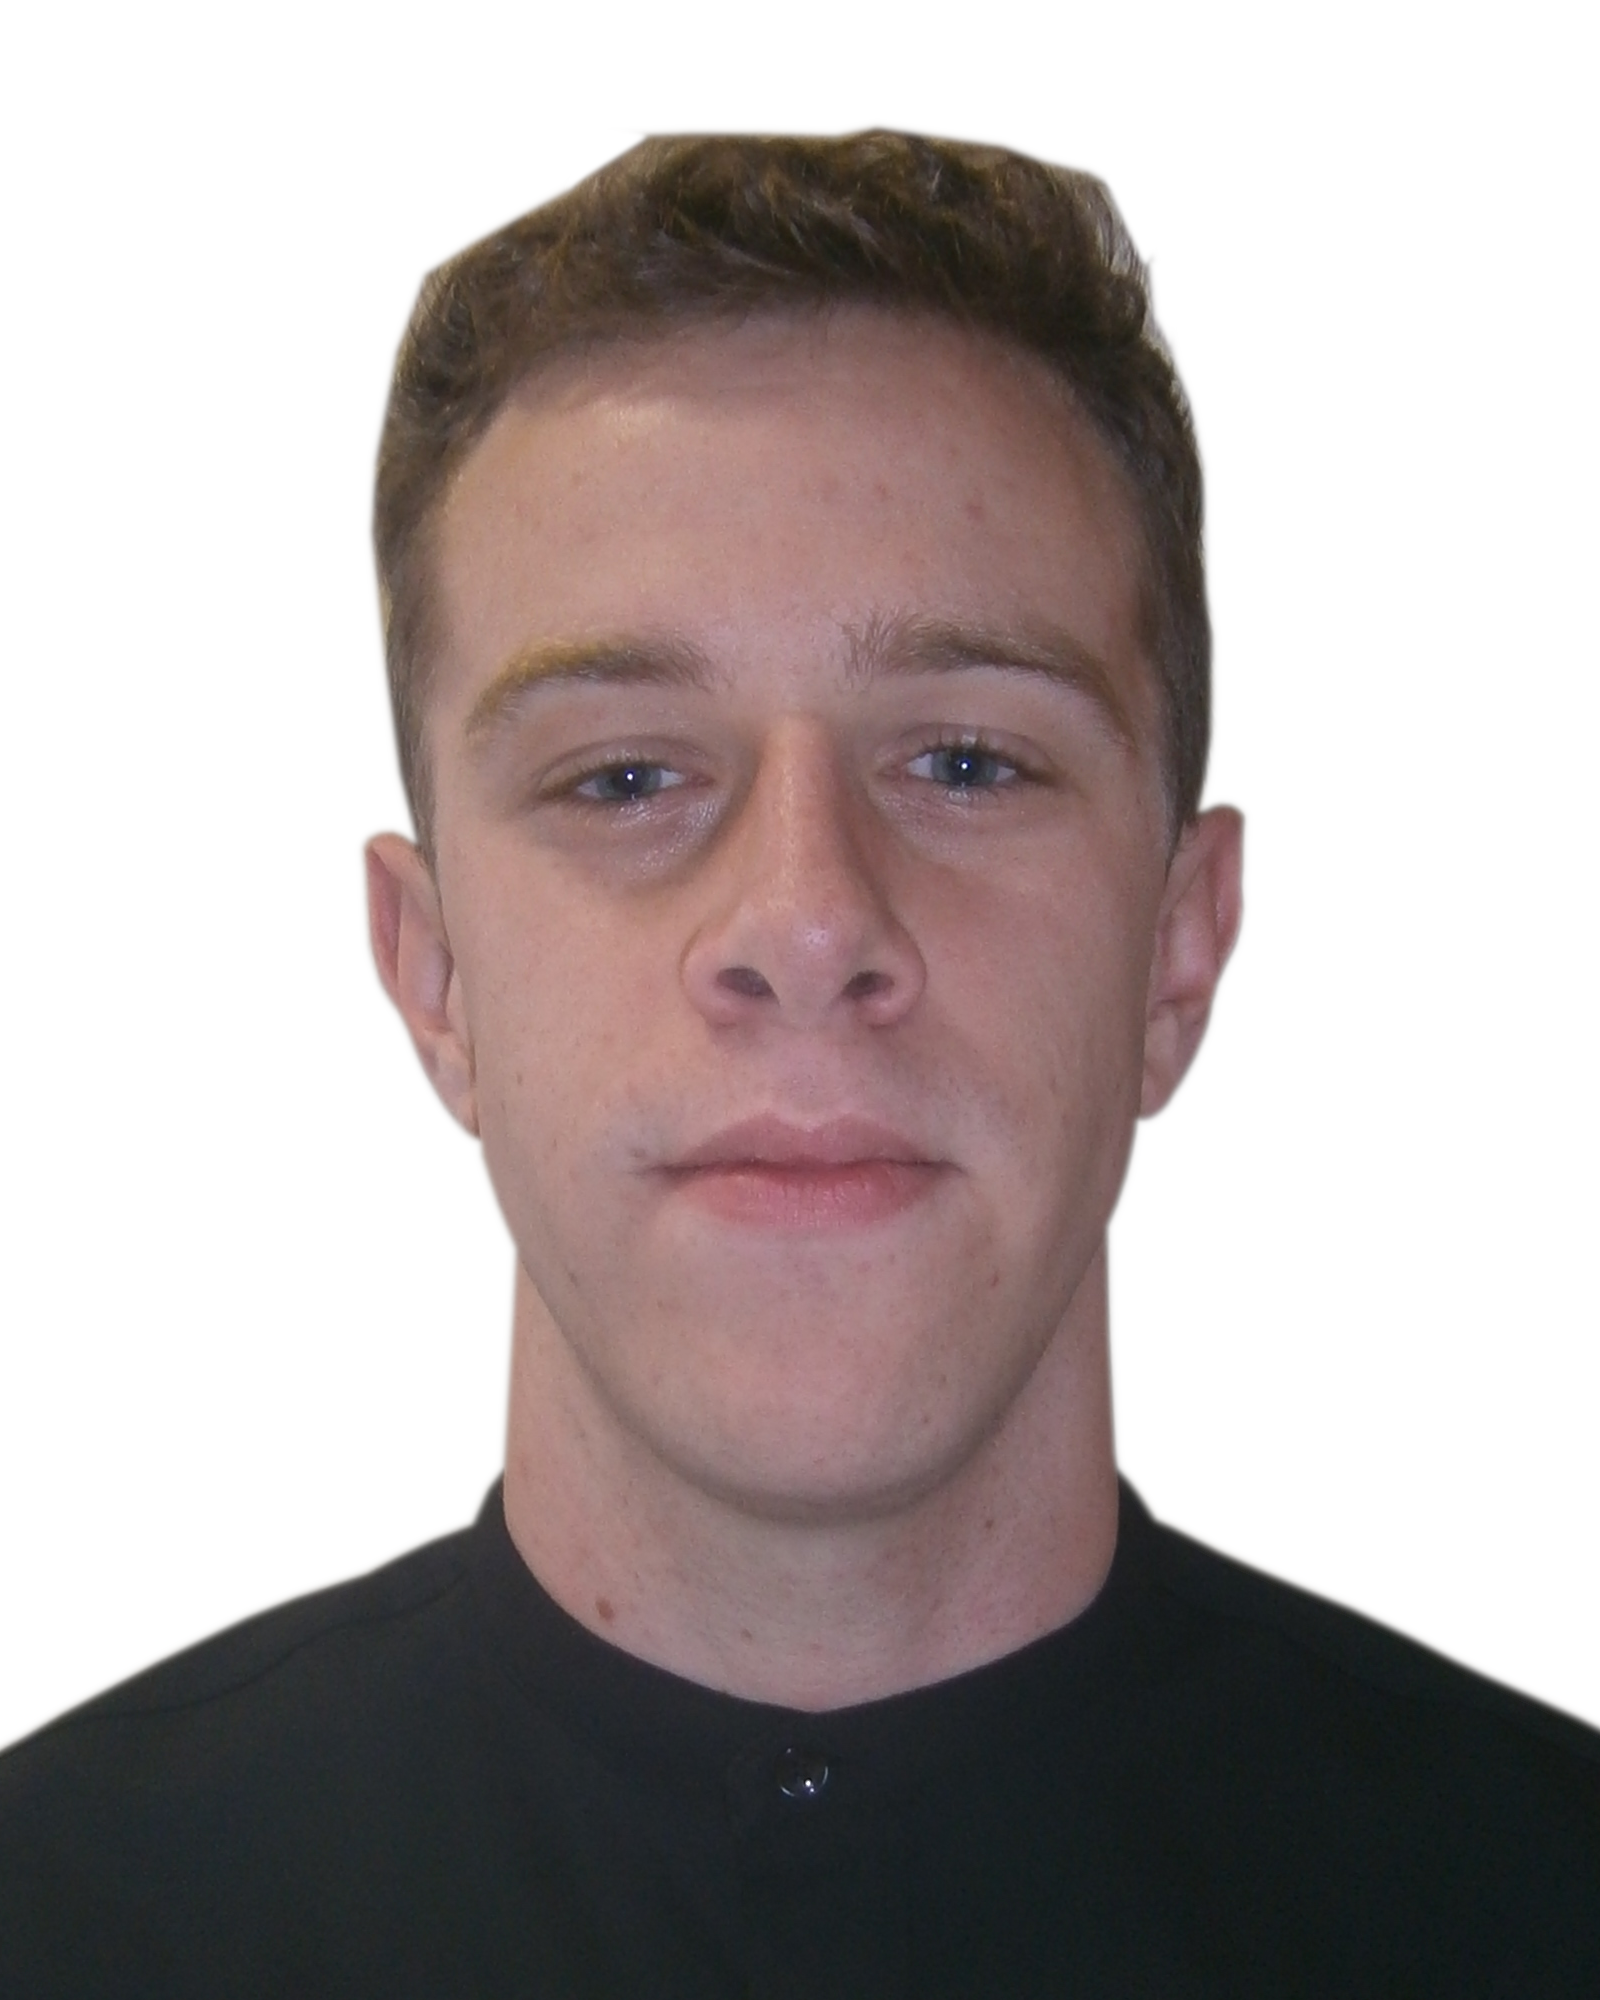
\includegraphics[width=1in,height=1.25in,clip,keepaspectratio]{Data/v4.png}}]{Josep Fanals i Batllori}
was born in la Bisbal d'Empordà, Spain, in 1998. He received the B.S. degree in electrical engineering from the Universitat de Girona, Girona, Spain, in 2020. His primary area of interest is the study of techniques to solve the power flow problem.
\end{IEEEbiography}

% if you will not have a photo at all:
\begin{IEEEbiography}[{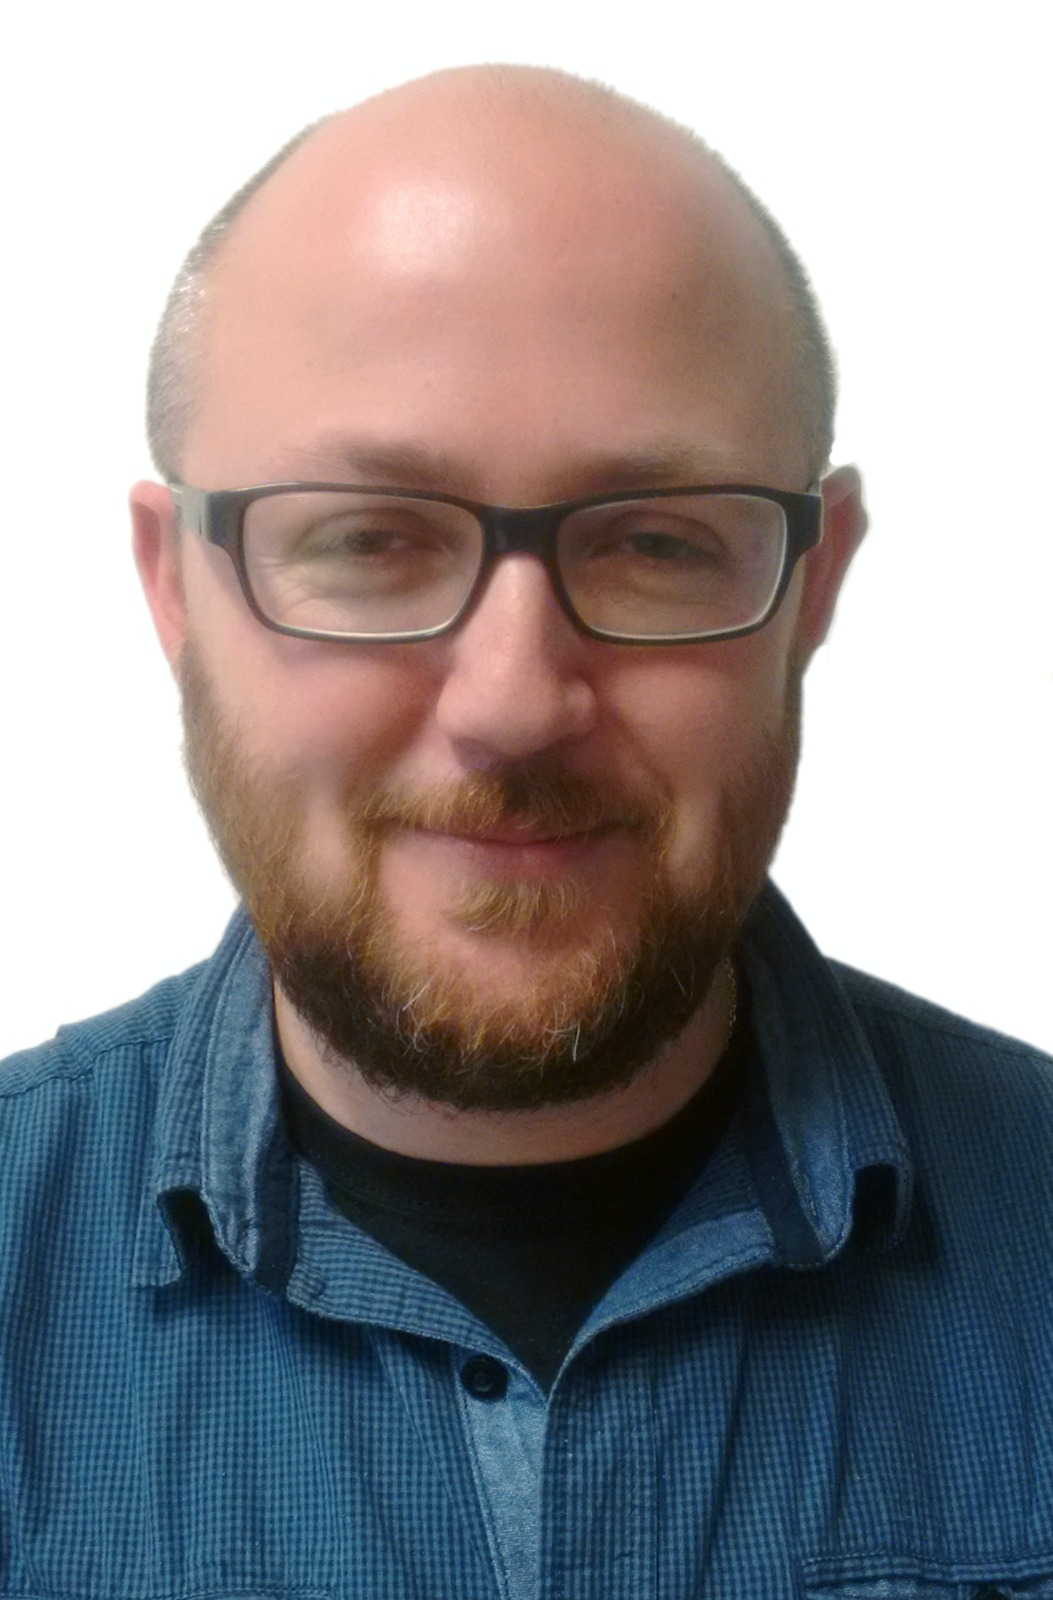
\includegraphics[width=1in,height=1.25in,clip,keepaspectratio]{Data/foto_SH.jpg}}]{Sergio Herraiz Jaramillo}
was born in Barcelona, Spain, in 1972. He received the B.S. degree in industrial engineering and the Ph.D. degree in engineering from the Universitat Politècnica de Catalunya, Barcelona, Spain in 1997 and 2002, respectively. Currently, he is a lecturer at the Institute of Informatics and Applications of the Universitat de Girona, Girona, Spain. His research interest is on power quality and energy effiency monitoring in power systems.
\end{IEEEbiography}

\vfill

% insert where needed to balance the two columns on the last page with
% biographies
%\newpage

% \begin{IEEEbiographynophoto}{Jane Doe}
% Biography text here.
% \end{IEEEbiographynophoto}

% You can push biographies down or up by placing
% a \vfill before or after them. The appropriate
% use of \vfill depends on what kind of text is
% on the last page and whether or not the columns
% are being equalized.

%\vfill

% Can be used to pull up biographies so that the bottom of the last one
% is flush with the other column.
%\enlargethispage{-5in}



% that's all folks
\end{document}


